\section{Appendix}



\section{VWM model}

\begin{notation}
	Treat 1D tensors as column vectors and 2D tensors as matrices, where appropriate.
	We use lower case to represent both 1D and 2D tensors but occasionally use upper case
	for 2D tensors where matrix operations are involved.
	
	\begin{enumerate}
		\item Let 
		$\Delta^d = \{ (x_0, x_1, \dots, x_d) : x_0 + x_1 + \dots + x_d = 1, x_i \ge 0, i = 0, 1, \dots, d\}$ denote the standard $d$-simplex.	
		
		\item  Let $\circ$ denote concatenation of two tensors with identical shape except possibly
		for their last dimensions $d_1$ and $d_2$, respectively,  
		resulting in a tensor with last dimension of $d_1+d_2$. 
		
		\item Let $\odot$ denote  element-wise product of two tensors of same shape,
		i.e., Hadamard product for vectors/matrices.
		
		\item Let $\otimes$ denote tensor product of two tensors, 
		i.e. Kronecker product for vectors/matrices.
	\end{enumerate}
\end{notation}	

\section{Basic layers/modules}

\colorbx{Linear (Affine) Layer}

\begin{description}
	\item[Inputs:] A tensor $x$ with last dimension $n$.
	\item[Parameter:] An affine function $\cG: \Reals^n \to \Reals^m$ with 
	weight and bias parameters.
	
	\item[Output:] A tensor $y$ with last dimension $m$, and remaining dimensions
	same as that of $x$, obtained by applying $\cG$ to each 1D slice of $x$
	along the last dimension.
\end{description}


\colorbx{Attention Module}

\begin{description}
	\item[Inputs:] 
	\begin{enumerate}
		\item[]
		\item Query: $q \in \Reals^d$
		\item Keys: $K \in \Reals^{N \times d}$	
		\item Values: $V \in \Reals^{N \times d}$. By default $V=K$, unless mentioned explicitly.	
	\end{enumerate}
	
	\item[Parameter:] Weight $w \in \Reals^d$
	
	\item[Outputs:] 
	\begin{enumerate}
		\item[]
		\item Content vector: $h =  V^{\T} u \in \Reals^d$
		\item Attention vector:  $w = \softmax(K(w \odot q)) \in \Reals^N$
	\end{enumerate}
\end{description}


\colorbx{Interaction Module}

\begin{description}
	\item[Inputs:] 
	\begin{enumerate}
		\item[]
		\item Base object: $b \in \Reals^d$
		\item Feature objects: $f \in \Reals^{M \times d}$	
	\end{enumerate}
	
	\item[Parameters:] 
	\begin{enumerate}
		\item[]
		\item Base object projection linear layer: $\cG: \Reals^d \to \Reals^d$
		\item Feature objects projection linear layer : $\cK: \Reals^{M \times d} \to \Reals^{M \times d}$
		\item Modifier linear layer:  $\cH: \Reals^{M \times 2d} \to \Reals^{M \times d}$	
	\end{enumerate}
	
	\item[Output:] Modified feature objects 
	$f' =  \cH( \cK(f) \odot ( \vone \otimes \cG(b))) \in  \Reals^{M \times d}$
\end{description}

\hrulefill

\section{VWM cell}

The VWM recurrent cell is executed for $T$ reasoning steps for every frame in
the temporal order.  Within a single frame, the cell state at the end of each reasoning step 
$t=1,2, \dots, T$ is denoted by $(c_t, M_t, o_t)$, where: 
\begin{enumerate}
	\item $c_t \in \Reals^d$ is the control state;
	\item $M_t \in  \Reals^{N \times d}$ is the visual working memory with $N$ slots;
	\item $w_t \in  \Reals^N$ is the write head; and
	\item $so_t  \in \Reals^d$ is the summary visual object.
\end{enumerate} 
The initial state is such that both $c_0$ and $so_0$ are initialized
to a fixed value at the start of each frame. However $M_0$ is initialized only once at
the start of the first frame and otherwise taken to be the value of $M_T$ at the
end of the previous frame.

%The number of slots $N$ for the VWM $M_t$ is not fixed because the neural network 
%parameters do not depend on it. It can be variable across the different datasets used
%for training, validation and test as well as within each dataset. This, for example, enables a 
%form of transfer learning where we can train on an easy dataset for one value of $N$
%and study its generalization to a hard dataset using a larger value of $N$.

\colorbx{Question-driven Controller}

The Question-driven Controller plays an important role in the reasoning process.
It drives the attention over the question and produces the new control states. Each new control state defines a new reasoning operation. The inputs of this unit are the past control state, the question encoding and the contextual words (see Question Encoding Unit). It uses the dot product attention between the contextual words
and the combination of the past control states and the question encoding.  This attention layer produces the new control state.

This unit also outputs the temporal class weights that will be used in the Reasoning Unit. It gives access to a temporal information for the current words (last, latest, now, none temporal).

\begin{description}
	\item[Inputs:] 
	\begin{enumerate}
		\item[]
		\item Reasoning step $t = 1,2, \dots, T$
		\item Previous control state: $c_{t-1} \in \Reals^d$	
		\item Contextual words: $cw \in \Reals^{L \times d}$
		\item Question encoding: $q \in \Reals^d$
	\end{enumerate}
	
	\item[Parameters:] 
	\begin{enumerate}
		\item[]
		\item Reasoning step-dependent linear layer: $\cG_t: \Reals^d \to \Reals^d$, depending on $s$
		\item Concatenation linear layer: $\cH: \Reals^{2d} \to \Reals^d$
		\item Attention module $\cA$
		\item Temporal classifier:  $\cK: \Reals^d \to \Delta^3$. A two-layer feedforward
		network with ELU activation in the hidden layer of $d$ units.	
		The classes for the temporal context are labeled ``last'', ``latest'', ``now'', as well as 
		a fourth class label ``none`` indicating no temporal context.
		If $\tau \in \Delta^3$ is the output of the classifier, we denote the components by
		$\tlast$, $\tlatest$, $\tnow$ and $\tnone$.
	\end{enumerate}
	
	\item[Outputs:] 
	\begin{enumerate}
		\item[]
		\item Control state $c_t \in \Reals^d$
		\item Control attention $ca_t \in \Reals^L$
		\item Temporal class weights $\tau_t \in \Reals^4$
	\end{enumerate}
	
	\item[Equations:] 
	\begin{enumerate}
		\item[]
		\item Modulation: $y = \cH\bigl([c_{t-1}, \cG_t(q)]\bigr)$
		\item Control state and attention: $c_t,  ca_t= \cA(y, cw)$
		\item Temporal classification: $\tau_t = \cK(c_t)$
	\end{enumerate}
\end{description}


\colorbx{Visual Retrieval Unit}

The visual retrievial unit is responsible to extract visual information from the current image given a control state coming from the Question-driven Controller. It is first projecting the past summary object and the feature maps together using the interaction module.
It is then using the attention module as follow. The query are the control states and the keys and are the feature maps coming from the image encoder. The results of this attention is applied on the modified features maps coming from the interaction module.  
This unit outputs the extracted object and the visual attention.

\begin{description}
	\item[Inputs:] 
	\begin{enumerate}
		\item[]
		\item Control state: $c_t \in \Reals^d$	
		\item Previous summary object: $so_{t-1} \in \Reals^d$
		\item Feature map of current frame: $F \in \Reals^{H \times W \times d}$
	\end{enumerate}
	
	\item[Parameters:] 
	\begin{enumerate}
		\item[]
		\item Interaction module $\cI$
		\item Attention module $\cA$
	\end{enumerate}
	
	\item[Outputs:] 
	\begin{enumerate}
		\item[]
		\item Visual object: $vo_t \in  \Reals^d$
		\item Visual attention: $va_t  \in \Reals^{H \times W \times d}$
	\end{enumerate}
	
	\item[Equations:]
	\begin{enumerate}
		\item[]
		\item Modified feature map: $\hat{F} = \cI(so_{t-1}, F)$
		\item Visual object and attention: $vo_t, va_t = \cA(y, \hat{F}, M_{t-1})$
	\end{enumerate}
\end{description}

\begin{note}
	Appropriate flatten/unflatten operations are performed to match the signature 
	of the modules.
\end{note}


\colorbx{Memory Retrieval Unit}

The role of the memory retrieval unit is to read and extract object from memory).
As the Visual Retrieval Unit, it uses the combination of the two following submodules. The interaction module blends together the extracted object and the content of the memory. The attention module then extract the corresponding object in memory if present. This unit outputs the extracted object and its corresponding location, we call it the "read head".

\begin{description}
	\item[Inputs:] 
	\begin{enumerate}
		\item[]
		\item Control state: $c_t \in \Reals^d$	
		\item Previous summary object: $so_{t-1} \in  \Reals^d$
		\item Previous VWM $M_{t-1} \in \Reals^{N \times d}$
	\end{enumerate}
	
	\item[Parameters:] 
	\begin{enumerate}
		\item[]
		\item Interaction module $\cI$
		\item Attention module $\cA$
	\end{enumerate}
	
	\item[Outputs:] 
	\begin{enumerate}
		\item[]
		\item Memory object: $mo_t \in \Reals^d$
		\item Read head: $\rhead_t \in \Reals^N$
	\end{enumerate}
	
	\item[Equations:]
	\begin{enumerate}
		\item[]
		\item Modified VWM: $\hat{M}_t = \cI(so_{t-1}, M_{t-1})$
		\item Memory object and attention: $mo_t, \rhead_t = \cA(y, \hat{M}_t, M_{t-1})$
	\end{enumerate}
\end{description}


\colorbx{Reasoning Unit}

%control_state, visual_object, memory_object, temporal_class_weights

\begin{description}
	\item[Inputs:] 
	\begin{enumerate}
		\item[]
		\item Control state: $c_t \in \Reals^d$
		\item Visual object: $vo_t \in \Reals^d$
		\item Memory object: $mo_t \in \Reals^d$
		\item Temporal class weights $\tau \in \Delta^3$
	\end{enumerate}
	
	\item[Parameters:] Validator modules $\cG, \cK: \Reals^{2d} \to \Reals$.
	Both $\cG, \cK$ are two-layer networks of $2d$ hidden units,
	using ELU activation in the hidden layer, and sigmoid in the output layer.
	
	\item[Output:] Predicate gates for the current reasoning step
	\begin{enumerate}
		\item Object match predicate gates (i) image: $\imatch_t \in [0,1]$ and 
		(ii) memory: $\mmatch_t \in [0,1]$.
		
		\item Memory update predicate gates (i) add: $\doadd_t \in [0,1]$ and
		(ii) replace: $\doreplace_t \in [0,1]$
	\end{enumerate}
	
	\item[Equations:]
	\begin{enumerate}
		\item[]
		\item $\imatch_t \in [0,1]$:
		It's true if there is a valid visual object. This assumes that
		the current reasoning step refers to either ```now''  or ``latest''.
		
		\item$\mmatch_t \in [0,1]$:
		It's true if there is a valid memory object. This assumes that
		the current reasoning step refers to either ``last'',  or alternatively ``latest'' 
		but there is no matching visual object.
		
		\item $\doadd_t$:
		
		
		\item $\doreplace_t$: 
	\end{enumerate}
\end{description}


\colorbx{Memory Update Unit}

This unit is meant to update the content of the memory. 

Three actions can happen:

\begin{itemize}
	\item There is no object to be added to memory, the memory remains unchanged
	\item There is one object that needs to be added to memory, but a similar object is already in memory at a given location. The new object will replace the old object at this location
	
	\item There is one object that needs to be added to memory, and  it is a new object. It is added at the write head location.
\end{itemize}


This module also updates the position of the write head. If a new object as been added to the current write head position, the right head shifts right to a new empty slot. If the object has been replaced, the write head doesn't move.
% visual_object, visual_working_memory, read_head, write_head, do_replace, do_add_new

\begin{description}
	\item[Inputs:] 
	\begin{enumerate}
		\item[]
		\item Visual object: $vo_t \in \Reals^d$
		\item Memory object: $mo_t \in \Reals^d$
		\item Memory update predicate gates:  $\doadd_t, \doreplace_t \in [0,1]$
		\item Read head: $\rhead_t \in \Reals^N$
		\item Previous VWM $M_{t-1} \in \Reals^{N \times d}$
		\item Previous write head: $\whead_{t-1} \in \Reals^N$
	\end{enumerate}
	
	\item[Outputs:] 
	\begin{enumerate}
		\item[]
		\item VWM $M_t \in \Reals^{N \times d}$
		\item Read head: $\rhead_t \in \Reals^N$
		\item Write head: $\whead_t \in \Reals^N$
	\end{enumerate}
	
\end{description}



\colorbx{Summary Object Update Unit}

The  Summary Unit is the last unit of the SAMCell. It is responsible to output the new summary object. It first picks which object is relevant between the object extracted from memory and the visual object extracted from the image. Once the relevant object is picked, it is combined with the former summary object through a linear layer to become the new summary object. It is the final step of the SAMCell reasoning cycle. 

The image encoder, question encoder and output unit are described in the appendix.

\begin{description}
	\item[Inputs:] 
	\begin{enumerate}
		\item[]
		\item Previous summary object: $so_{t-1} \in \Reals^d$
		\item Visual object: $vo_t \in \Reals^d$
		\item Memory object: $mo_t \in \Reals^d$
		\item Object predicate gates: $\imatch_t, \mmatch_t \in [0,1]$
	\end{enumerate}
	
	\item[Parameters:] Concatenation linear layer $\cH$ 
	
	\item[Output:] 
	New summary object:
	$so_t = \cH\bigl([so_{t-1}, (\imatch_t * vo_t + \mmatch_t * mo_t)]\bigr) \in \Reals^d$ 
	
\end{description}


\noindent\makebox[\linewidth]{\rule{\paperwidth}{1pt}}



\begin{figure}
	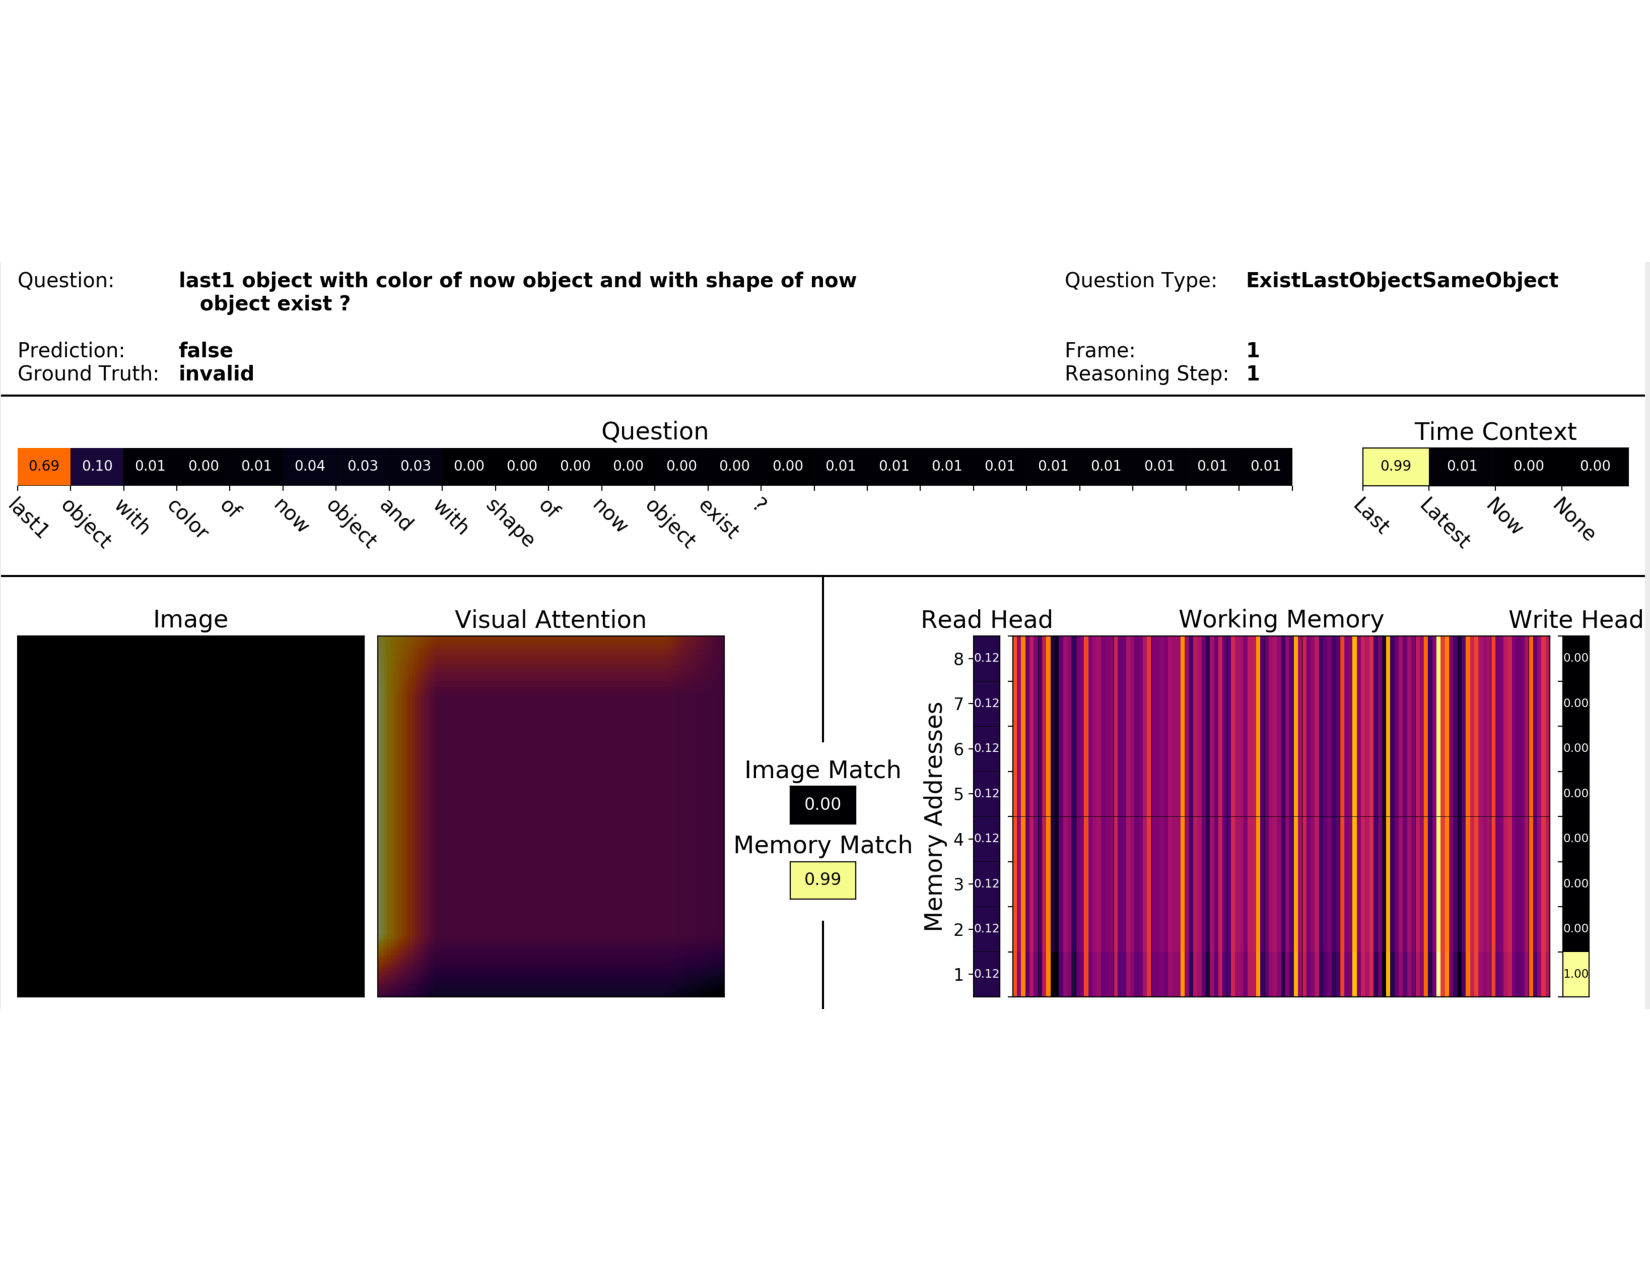
\includegraphics[width=\textwidth]{img/model2}
	\label{fig:model}
\end{figure}	

\begin{figure}
	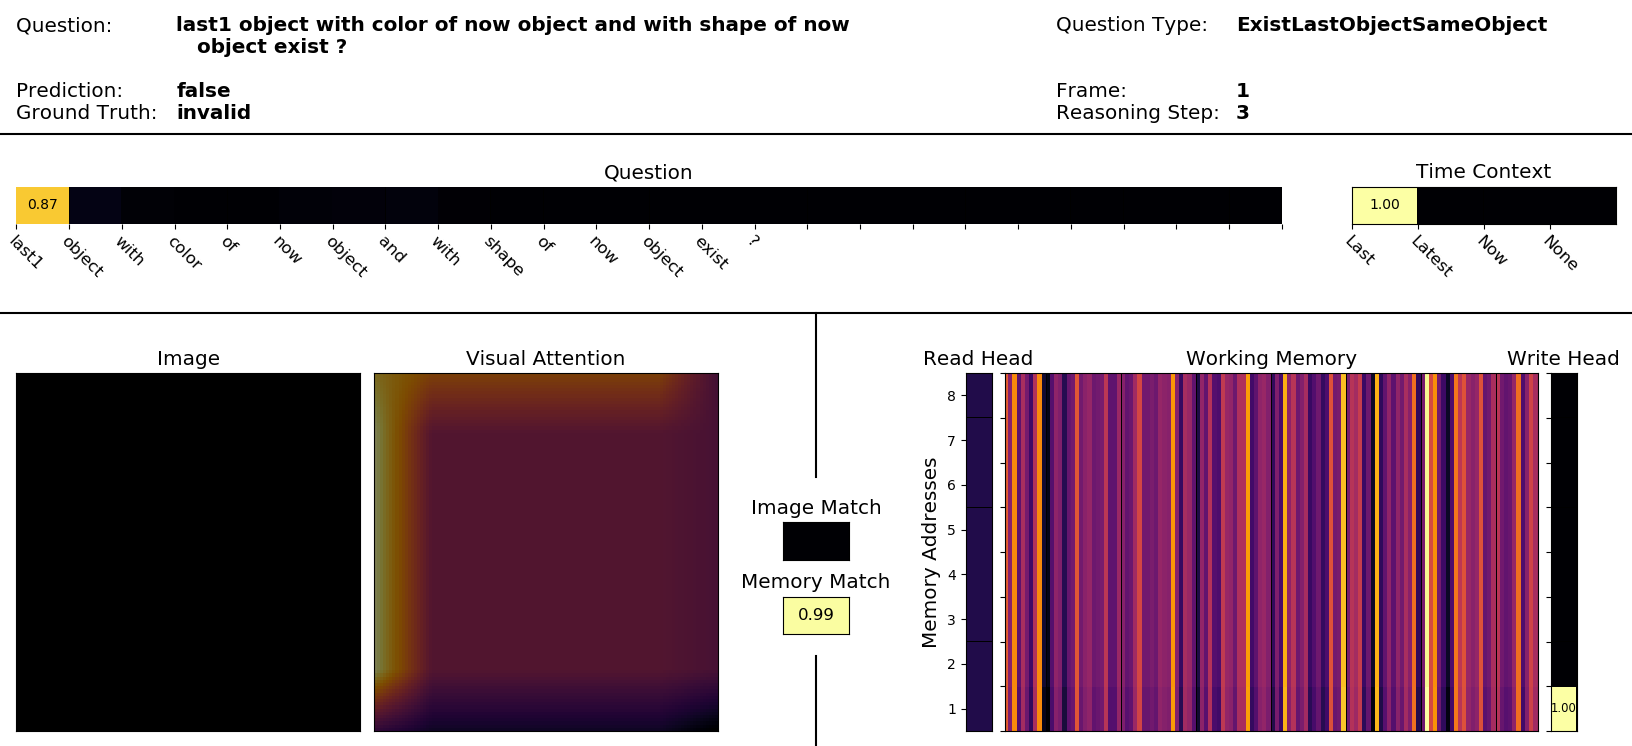
\includegraphics[width=\textwidth]{img/image}
	\label{fig:model}
\end{figure}	

\colorbx{Image Encoder}

\colorbx{Question Encoder}

\colorbx{Output Unit}



\section{Training and Implementation Details}


\subsection{Training and testing Methodology}

SAMNet is implemented on IBM's Mi-Prometheus~\cite{kornuta2018accelerating} framework based on Pytorch. 
We trained all our models using NVIDIA’s GeForce GTX TITAN X GPUs. SAMNet was trained using 8 reasoning steps and a hidden state size of 128. The external memory has 128-bit slots for all experiments. We trained our model until convergence but we also have set a training time limit of 80 hours.

We compared our model to the original COG model  ~\cite{yang2018dataset} using their implementation (https://github.com/google/cog) and scores provided by the authors through personal communications. We used the same training parameters detailed in the original paper and reproduced their results.  For the generalization experiments from canonical to hard, we used the verified model and obtained new results that were not reported in the reference paper.   In Table 1 COG section shows 4 columns divided into two parts: "paper" and "ours" which distinguish between the results reported in the paper vs. our own experiments.

Our experiments focused on the 22 classification tasks provided by the COG dataset.  First we evaluated SAMNet's performance on the canonical setting and compared it with the COG Model. As shown in Table 1 we could achieve a small improvement in accuracy, from 97.6\% for the COG model to 98\% for SAMNet. Next we focused on the hard setting of the dataset which increases the number of distractors from 1 to 10 and the number of frames from 4 to 8.

The first approach was to train a model on the hard training set, and test it on the hard test set. This is the same approach used by the COG paper ~\cite{yang2018dataset} to evaluate performance on the hard dataset. We achieve a test accuracy of 91.9 \% which represents a 12\% improvement from the COG model score (see Table 1).
%It shows that SAMNet's design choices make a difference when it come to harder tasks with longer sequences and more distractors objects.

The second approach was to see if the models can generalize from the easy to the hard setting. For this experiment, we trained a model on the canonical dataset, and directly tested on the hard dataset.  This experiment highlighted the most significant difference between SAMNet and the baseline COG model.

Finally we trained a model on the canonical data set, fine-tuned it on the hard data set using only 25k iterations, and tested on the hard dataset. Thanks to fine-tuning, we can observe a significant improvement from 91.6\%  to 96.5\% test accuracy which represents the state of the art accuracy for the hard setting (classification tasks).
After a short fine-tuning process, the transferred model could generalize well to harder tasks and even surpass the accuracy obtained in the first approach. We note that the third approach is also twice faster than the first one, and it is more effective in terms of accuracy.

A more granular analysis of accuracy per task shows a major improvement for the two hardest tasks, AndCompareShape and AndCompareColor. Those two tasks represent a higher level of difficulty due to the number of objects to be remembered in order to answer the question correctly.
As we can see in Table 2 we could achieve a 12\% improvement for the canonical data set and almost a 40\% improvement for the hard dataset.
The large improvement in these memory-intensive tasks indicate that the SAMNet's external memory plays a crucial role in our results. 
The training and implementation details are in appendix.








\begin{table}[t]
	\tiny
	
	\caption{COG test set accuracies for  SAMNet \& COG models. For the COG section, the results marked as 'paper' comes from the original COG paper ~\cite{yang2018dataset}, whereas the results marked as 'ours' come from our own experiments using the following implementation: https://github.com/google/cog }
	
	\resizebox{\textwidth}{!}{
		\centering
		\begin{tabular}{ccccccccccc}
			\toprule
			Model & & SAMNet & && && COG&& \\
			\cmidrule{2-5} \cmidrule{7-11} 
			&&&&& & paper & ours & ours & paper&\\
			\cmidrule{7-9} \cmidrule{10-11}
			Trained on       & canonical & canonical & canonical & hard &           &  canonical  & canonical  & canonical & hard \\ 
			Fine tuned on  & - & - & hard  & - &           & -   & - & hard & - \\ 
			Tested on        & canonical & hard & hard & hard &            &canonical  & hard & hard & hard  \\ 
			\midrule
			
			Overall accuracy & 98.0 & 91.6 & 96.5  & running &           & 97.6  & 65.9 & running& 80.1 \\ 
			
			\midrule 
			
			
			AndCompareColor	&	93.5		&	82.7	&	89.2	&&		&81.9	&57.1&&	51.4
			\\ 
			AndCompareShape	&	93.2 		&	83.7	&	89.7	&&	&	80.0	&53.1	&&50.7\\ 
			AndSimpleCompareColor	&	99.2	&		85.3	&	97.6	&	&	&99.7&	53.4&&	78.2\\ 
			AndSimpleCompareShape	&	99.2&			85.8	&	97.6	&&	&	100.0	&56.7&&	77.9\\ 
			CompareColor	&	98.1		&	89.3	&	95.9	&&		&99.2&	56.1&&	50.1\\ 
			CompareShape	&	98.0	&		89.7	&	95.9	&&	&99.4	&66.8	&&50.5
			\\ 
			Exist	&	100.0	&		99.7	&	99.8		&&	&	100.0&	63.5&&	99.3\\ 
			ExistColor	&	100.0		&	99.6	&	99.9	&&	&	99.0&	70.9&&	89.8\\ 
			ExistColorOf	&	99.9	&		95.5	&	99.7		& & &	99.7&	51.5&&	73.1\\ 
			ExistColorSpace	&94.1		&	88.8	&	91.0	&& &	98.9	&72.8	&&89.2\\ 
			ExistLastColorSameShape	&	99.5		&	99.4	&99.4	&&		&100.0	&65.0&&	50.4
			\\ 
			ExistLastObjectSameObject	&	97.3	&		97.5	&	97.7	&&	&	98.0&	77.5	&&60.2\\ 
			ExistLastShapeSameColor	&	98.2		&	98.5&	98.8	&&	&	100.0&	87.8&&	50.3\\ 
			ExistShape	&	100.0	&	99.5	&	100.0	&&&	100.0&	77.1	&&92.5\\ 
			ExistShapeOf	&	99.4		&	95.9	&	99.2	&&&100.0	&52.7&&89.8\\ 
			ExistSpace	&	95.3	&	89.7	&	93.2	&&		&	98.9	&71.1	&&92.8\\ 
			GetColor	&	100.0		&	95.8&	99.9	&& &	100.0&	71.4&&	97.9\\ 
			GetColorSpace	&	98.0		&	90.0	&	95.0&	& &	98.2	&71.8&&	92.3\\ 
			GetShape	&	100.0		&	97.3&	99.9&	&	&	100.0  &83.5&&	97.1
			\\ 
			GetShapeSpace	&	97.5	&	89.4	&	93.9	&&&	98.1  &78.7	&&	90.3\\ 
			SimpleCompareShape	&	99.9		&	91.4	&	99.7	&	&&	100.0 & 67.7&&	99.3\\ 
			SimpleCompareColor	&	100.0 		&	91.6  &	99.80&	&	&	100.0&	64.2&&	99.3	  \\ 
			
			
			
			
			
			
			
			\bottomrule
		\end{tabular}
	}
	
	\label{results}
\end{table}



\begin{table}[!t]
	\centering
	\caption{COG Dataset parameters for the canonical setting and the hard setting  }
	\resizebox{\textwidth}{!}{
		
		
		\begin{tabular}{ccccccc}
			\toprule
			
			Dataset    &  	number of frames  &  	maximum memory duration & number of distractors & size of training set & size of validation/test set    \\ 
			\midrule
			
			Canonical setting & 4 & 3 & 1 & 10000320 & 500016 &   \\
			\midrule
			
			Hard  setting & 8 & 7& 10 & 10000320 & 500016  \\
			\bottomrule
			
		\end{tabular}
	}
	
	
	\label{tab:parameters}
\end{table}


